\documentclass{beamer}
\usepackage[utf8]{inputenc}
\usepackage{amsmath}
\usepackage{amsfonts}
\usepackage{amssymb}
\usepackage{graphicx}
\usepackage{polski}
\usepackage{tikz}
\usepackage{calc}
\usepackage{array}

\usetikzlibrary{positioning}
\usetheme{Warsaw}

\title[Biuro~matrymonialne]{System ekspertowy realizujący zadania biura matrymonialnego}
\subtitle{Opis teoretyczny projektu}
\author[Bułka,~Byczyńska,~Czyżniejewski,~Rymuszka]{Aleksandra~Bułka\\Aleksandra~Byczyńska\\Jakub~Czyżniejewski\\Mateusz~Rymuszka}
\institute[MiNI~PW]{Wydział Matematyki i Nauk Informacyjnych\\Politechnika Warszawska}
\date[lato~2019]{\today}

\begin{document}
 
\frame{\titlepage}

\begin{frame}
	\frametitle{Konspekt}
	
	\tableofcontents
	
\end{frame}

\section{Założenia projektowe}

\subsection{Porównanie: kiedyś i dzisiaj}

\begin{frame}

	\begin{block}{Dawniej}
		Pracownik biura matrymonialnego (tutaj: ekspert dziedziny), na podstawie opisu wymagań klienta, odszukiwał osoby, które pasowałyby do preferencji osoby poszukującej partnera
	\end{block}

	\begin{figure}
		\centering
		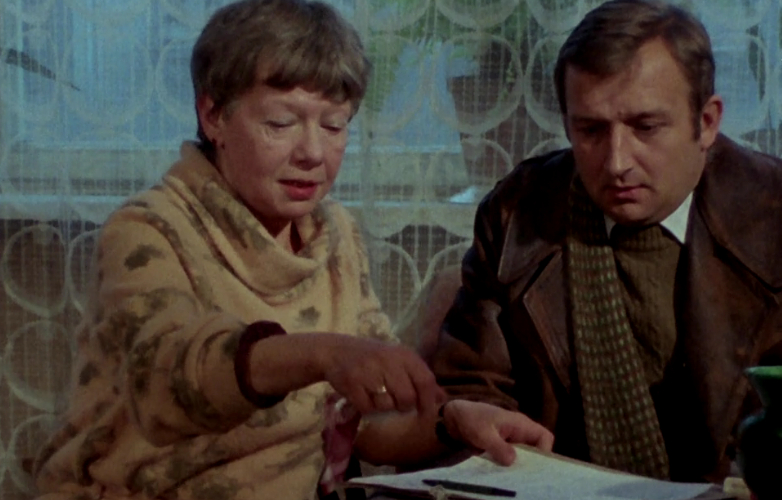
\includegraphics[height=0.5\textheight,keepaspectratio]{images/biuro-kiedys.jpg}
		\caption{Kadr z serialu ``Jan Serce``}
	\end{figure}

\end{frame}

\begin{frame}

	\begin{block}{Dawniej}
		Pracownik biura matrymonialnego (tutaj: ekspert dziedziny), na podstawie opisu wymagań klienta, odszukiwał osoby, które pasowałyby do preferencji osoby poszukującej partnera
	\end{block}
	
	\begin{block}{Wady}
		\begin{itemize}
			\item możliwość zgubienia lub przeoczenia karty klienta
			\item długi czas odszukiwania osób pasujących do rysopisu
			\item subiektywizm osoby wertującej kartotekę
			\item brak powtarzalności procesu
		\end{itemize}
	\end{block}

\end{frame}

\begin{frame}
	
	\begin{block}{Dzisiaj}
		System ekspertowy, po wypełnieniu kwestionariusza przez klienta, automatycznie dopasowuje potencjalnych kandydatów do randkowania
	\end{block}
	
	\begin{figure}
		\centering
		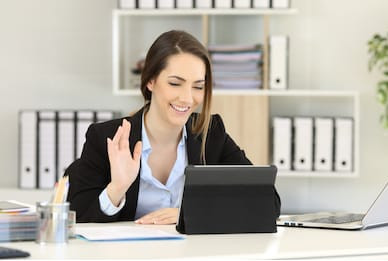
\includegraphics[height=0.5\textheight,keepaspectratio]{images/biuro-dzisiaj.jpg}
		\caption{Biuro matrymonialne obecnie}
	\end{figure}

\end{frame}

\begin{frame}
	
	\begin{block}{Dzisiaj}
		System ekspertowy, po wypełnieniu kwestionariusza przez klienta, automatycznie dopasowuje potencjalnych kandydatów do randkowania
	\end{block}
	
	\begin{block}{Zalety wobec starego systemu}
		\begin{itemize}
			\item wszyscy klienci biura są uwzględnieni 
			\item krótki czas wnioskowania
			\item bezstronność komputera
			\item dyskrecja
		\end{itemize}
	\end{block}

\end{frame}

\subsection{Wymagania biznesowe}

\begin{frame}
	
	\begin{block}{Wymagania biznesowe}
		\begin{itemize}
			\item możliwość natychmiastowego dodawania/edycji/usuwania klientów z bazy biura
			\item wybór najtrafniejszej osoby według preferencji klienta
			\item prezentacja osób spełniający wymagania postawione w formularzu
			\item niezależność logiki wnioskowania od bazy wiedzy
			\item jasny i przejrzysty interfejs użytkownika
		\end{itemize}
	\end{block}

\end{frame}

\section{Opis architektury systemu}

\subsection{Schemat architektury}

\begin{frame}
    \begin{figure}
		\centering
		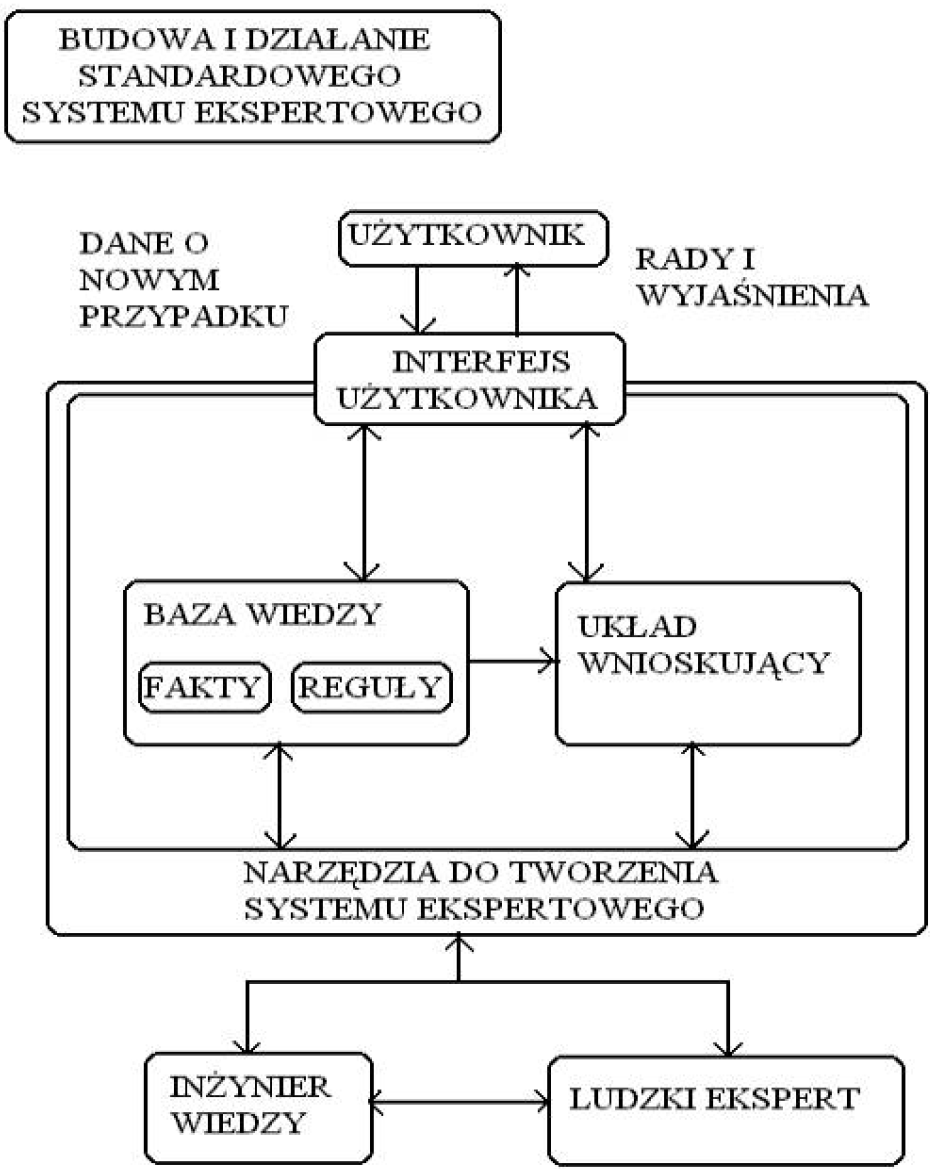
\includegraphics[height=0.85\textheight,keepaspectratio]{images/diagram.png}
		\caption{diagram z materiałów z wykładu}
	\end{figure}
	
\end{frame}

\subsection{Opis modułów systemowych}

\begin{frame}

	\begin{block}{Moduły wnioskowania}
		Moduły wnioskowania będą zawierać klauzule definiujące fakty i reguły odpowiadające za wnioskowanie na podstawie bazy wiedzy. 
		
		Zespół zaimplementuje:
		\begin{itemize}
		    \item moduł wnioskowania nierozmytego - wyznaczający reguły decyzyjne w oparciu o logikę boolowską
			\item moduł wnioskowania rozmytego - wyznaczający reguły decyzyjne w oparciu o logikę rozmytą
		\end{itemize}
		
		Każdy profil będzie zawierał cechy rozmyte (np. \textit{atrakcyjność}) i nierozmyte (np. \textit{płeć}). Użytkownik będzie określał swoje preferencje korzystając moduł użytkownika.
	\end{block}

\end{frame}

\begin{frame}

	\begin{block}{Baza wiedzy}
		Osobny moduł będzie stanowiła baza wiedzy. Można podzielić ją na:
		\begin{itemize}
			\item część statyczną, z podstawowymi faktami i regułami na temat systemu
			\item część dynamiczną, ładowaną z pliku lub modyfikowaną przez obsługującego (moduł eksperta)
		\end{itemize}
		Zespół przygotuje zarówno predykaty statycznej bazy wiedzy oraz interfejs do zarządzania dynamiczną bazą danych.
	\end{block}

\end{frame}

\begin{frame}
	
	\begin{block}{Interfejs eksperta}
		Prosty (tekstowy) interfejs eksperta. Będzie umożliwiał:  
		\begin{itemize}
		    \item interakcję z ekspertem
		    \item dodawanie, usuwanie, edycję profili kandydatów
		    \item sprawdzanie integralności danych w bazie
		    \item serializacja danych
		\end{itemize}
	\end{block}

\end{frame}

\begin{frame}
	
	\begin{block}{Interfejs użytkownika}
		Prosty (tekstowy) interfejs użytkownika. Będzie umożliwiał:  
		\begin{itemize}
		    \item interakcję z użytkownikiem
		    \item przeprowadzenie wnioskowania na podstawie wprowadzonych faktów
		    \item zwrócenie użytkownikowi profili najbardziej pasujących osób
		\end{itemize}
	\end{block}

\end{frame}

\section{Wnioskowanie}

\subsection{Metody wnioskowania}

\begin{frame}

	\begin{block}{Przykłady pytań rozmytych}
		\begin{itemize}
		    \item Wiek
	        \item Wzrost
            \item Lokalizacja
            \item Zainteresowania
            \item Atrakcyjność
            \item Gust muzyczny/filmowy/książkowy
            \item Marzenia/aspiracje
            \item Dochody
		\end{itemize}
	\end{block}

\end{frame}

\begin{frame}

	\begin{block}{Przykłady pytań nierozmytych}
		\begin{itemize}
		    \item Wykształcenie
            \item Płeć
            \item Orientacja seksualna
            \item Zawód
            \item Religia
		\end{itemize}
	\end{block}

\end{frame}

\subsection{Przykład działania programu}

\begin{frame}
    \begin{block}{Wprowadzona kwerenda}
		\begin{itemize}
		    \item Humanista (z wykształcenia)
		    \item Nie informatyk (zawód)
            \item Mężczyzna
            \item Około 0.75 atrakcyjności
            \item Młody (ok. 25 lat)
		\end{itemize}
	\end{block}
   
	\begin{figure}
		\centering
		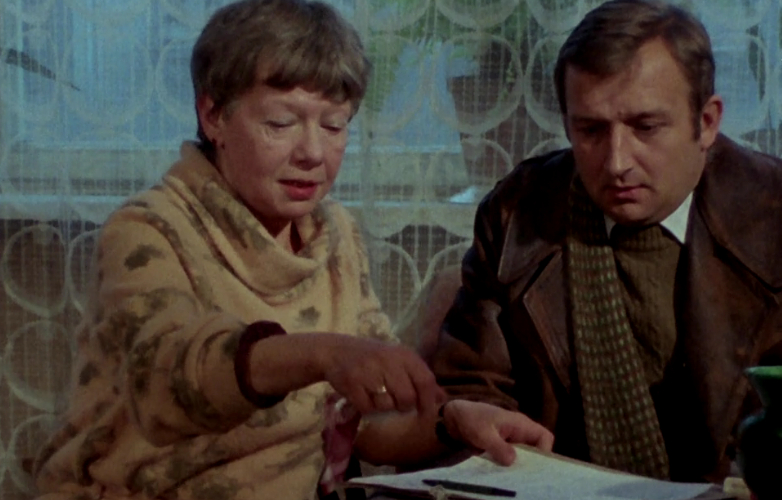
\includegraphics[height=0.3\textheight,keepaspectratio]{images/biuro-kiedys.jpg}
		\caption{Kadr z serialu ``Jan Serce``}
	\end{figure}

\end{frame} 

\begin{frame}

	\begin{block}{Przykładowy wynik}
		\begin{itemize}
		    \item 0.99 Marcel (wyk. filozofia, psycholog, 26 lat, 0.95 atrakcyjności)
		    \item 0.8 Michał (wyk. polityka, polityk, 29 lat,  0.99 atrakcyjność)
            \item 0.6 Stefan (wyk. politologia, data scientist, 20 lat, 0.6 atrakcyjności)
            \item 0.55 Józek (wyk. pedagogika, nauczyciel j. polskiego, 32 lata, 0.5 atrakcyjności)
		\end{itemize}
	\end{block}

\end{frame}

\end{document}
